\documentclass{article}
\usepackage{amsmath}
\usepackage{graphicx}
\usepackage{hyperref}

\title{Survey Report on Generative AI for Semantic Communication}
\author{Le Xia, Yao Sun, Chengsi Liang, Lei Zhang, Muhammad Ali Imran, Dusit Niyato}
\date{}

\begin{document}

\maketitle

\section{Introduction}

Semantic communication (SemCom) is an emerging paradigm that significantly saves spectrum resources and improves information interaction efficiency. However, current SemCom systems are limited by their lack of context reasoning and background knowledge provisioning. Generative Artificial Intelligence (GAI) technology, with its powerful capability in creating valuable, diverse, and personalized content, is considered to effectively enhance SemCom systems. This paper proposes a novel GAI-assisted Semantic Communication Network (GAI-SCN) framework to achieve more efficient and reliable semantic reasoning and resource utilization.

\section{Background}

Current SemCom systems are limited by their lack of context reasoning and background knowledge provisioning. Generative AI (GAI) shows great potential in generating multimodal content and understanding context, which can significantly improve the training efficiency, context reasoning ability, and spectrum utilization of semantic communication.

\section{Challenges}

\begin{itemize}
    \item \textbf{Data Requirements}: SemCom requires vast amounts of data for background knowledge construction and model pre-training.
    \item \textbf{Semantic Accuracy}: Existing systems lack accuracy in semantic calibration and recovery when dealing with complex contextual fragments.
    \item \textbf{Computational and Storage Resources}: Large GAI models (e.g., ChatGPT-3) require significant computational and storage resources.
    \item \textbf{Content Uncertainty and Delay}: GAI-generated content may introduce uncertainty and increase processing and dissemination delay.
\end{itemize}

\section{Solution}

A GAI-assisted Semantic Communication Network (GAI-SCN) framework is proposed, which collaborates across cloud, edge, and mobile layers, using global and local GAI models to enable multimodal semantic content provisioning, joint source-channel coding (JSCC), and AI-generated content (AIGC) acquisition, maximizing the efficiency and reliability of semantic reasoning and resource utilization.

\subsection{Model Selection}
\begin{itemize}
    \item \textbf{Local GAI Model}: ViT combined with GPT-2 for image-to-text conversion and keyword extraction.
    \item \textbf{Global GAI Model}: Stable Diffusion 2.1 for generating AI-generated images from prompts.
\end{itemize}

\subsection{Semantic Communication Setup}
\begin{itemize}
    \item Use deep convolutional network (Observation-Centric Sort) and Transformer-based semantic decoder for segmentation and recovery.
    \item Train models with additive white Gaussian noise channel at 0 dB SNR, testing with 327 images.
\end{itemize}

\subsection{Optimizer}
\begin{itemize}
    \item Adam optimizer with an initial learning rate of 5×10⁻⁴.
\end{itemize}

\subsection{Benchmarks}
\begin{itemize}
    \item \textbf{GAI-Assisted Traditional Communication}: Encodes AIGC into bits using predefined rules.
    \item \textbf{Typical SemCom}: Transmits original images solely through semantic coding models.
\end{itemize}

\section{Experimental Setup}

The experimental setup includes model selection, semantic communication setup, optimizer selection, and benchmarks. These settings validate the initial performance of the GAI-SCN framework in the task of image transmission.

\section{Results Analysis}

Fig. 5 shows that the complexity of images significantly impacts the recovery performance when using the GAI-SCN framework. Specifically, as the number of observable objects in the original images increases, semantic similarity decreases, object quantity discrepancy increases, and the recovery ratio of original objects declines. This demonstrates that the framework faces greater challenges in maintaining recovery accuracy and semantic consistency with more complex images.

\begin{figure}[h]
    \centering
    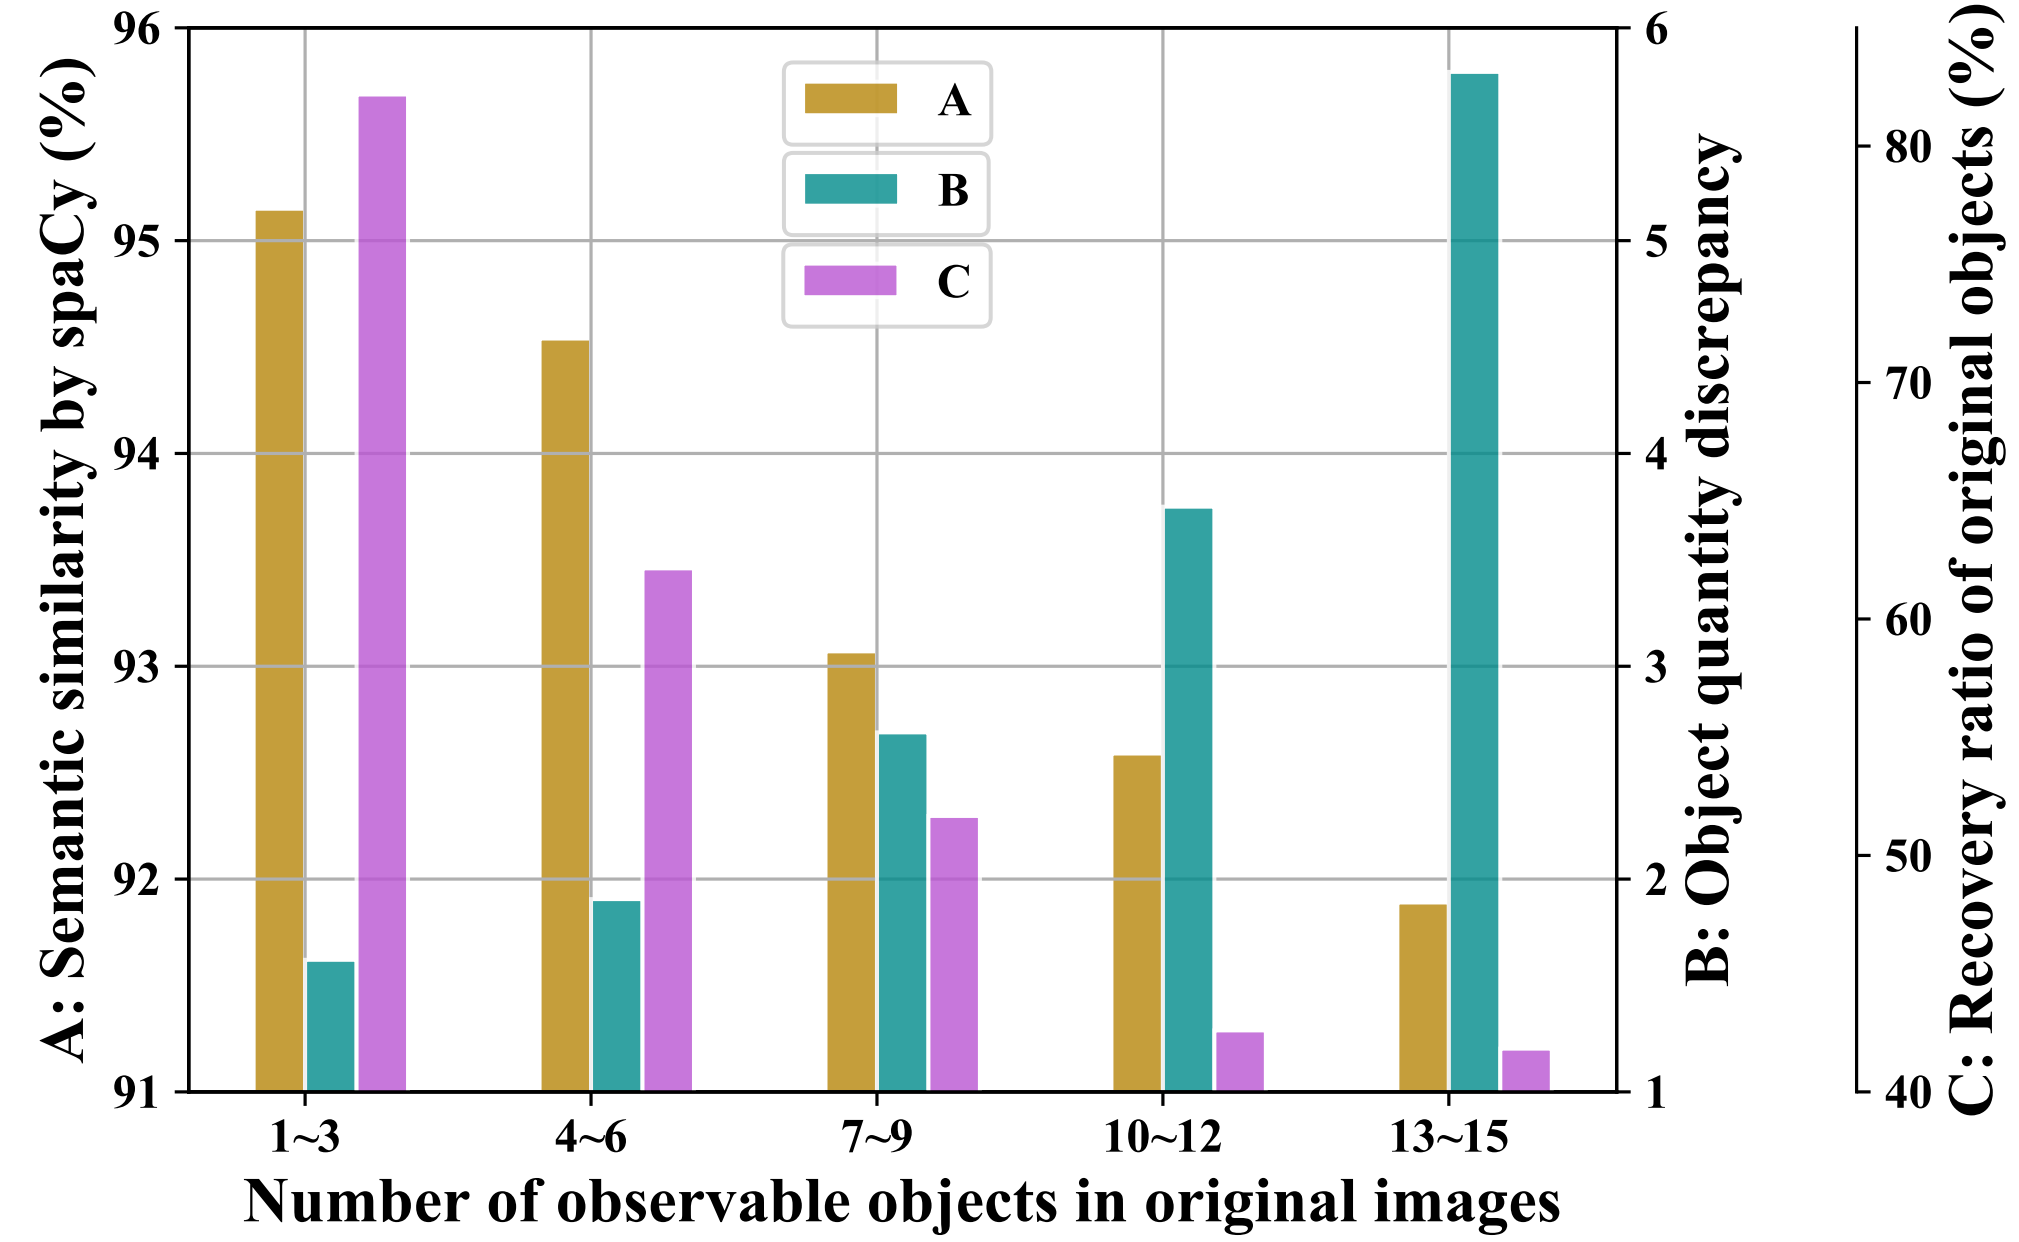
\includegraphics[width=\textwidth]{image.png}
    \caption{Comparisons between original and recovered images by the proposed GAI-SCN framework in terms of three metrics: A) Semantic similarity by spaCy; B) Object quantity discrepancy; C) Recovery ratio of original objects.}
\end{figure}

\section{Open Research Issues and Outlooks}

\begin{itemize}
    \item \textbf{Limited Device Resources}: Implementing sophisticated AI models on devices with limited storage, memory, and computational power.
    \begin{itemize}
        \item \textbf{Potential Solution}: Use model compression and acceleration techniques like knowledge distillation, parameter pruning, and quantization to reduce model complexity and size.
    \end{itemize}
    \item \textbf{Randomness in GAI Content}: Variability in AI-generated content and semantic decoder outputs, leading to inconsistencies.
    \begin{itemize}
        \item \textbf{Potential Solution}: Investigate granularity tuning for keyword extraction and semantic calibration to mitigate randomness.
    \end{itemize}
    \item \textbf{Inactive Sharing of Knowledge and Preferences}: Encouraging users to share personal preferences and background knowledge necessary for customized AI and SemCom services.
    \begin{itemize}
        \item \textbf{Potential Solution}: Develop incentive mechanisms, such as rewards or benefits, to motivate users to contribute their data for system improvements.
    \end{itemize}
\end{itemize}

\section{Conclusion}

Integrating generative AI with semantic communication offers a promising approach to enhancing communication efficiency and resource utilization. The GAI-SCN framework utilizes global and local GAI models to enable multimodal content provisioning, joint source-channel coding (JSCC), and AI-generated content (AIGC) acquisition, maximizing the efficiency and reliability of semantic reasoning and resource utilization, providing an innovative solution for future semantic communication networks.

\end{document}
